% Dokument:
\documentclass[a4paper,10pt,twocolumn]{article}
\usepackage[utf8]{inputenc}
%\usepackage[norsk]{babel}
\usepackage{hyperref}

% Formatering:
\usepackage{geometry,amsthm,blindtext}
\setlength{\parindent}{0mm}
\setlength{\parskip}{1.8mm}
% Symboler
\usepackage[geometry]{ifsym}
% Matematikk:
\usepackage{amsmath,mathtools,amsfonts,xparse,physics,esint,mathrsfs,nicefrac,siunitx}
% Kode:
\usepackage{verbatim,listings,algpseudocode}
% Tekst:
\usepackage{textcomp,varioref,enumerate,bbold}
% Figurer:
\usepackage{graphicx,subcaption,float,dcolumn,multirow}
\usepackage[section]{placeins}
% Farge:
\usepackage{xcolor}

% Dcolumn-kolonner
\newcolumntype{,}{D{,}{{,}}{2}}
\newcolumntype{=}{D{=}{=}{-1}}
\newcolumntype{.}{D{.}{{.}}{2}}
\newcolumntype{C}{>{$}c<{$}}

% Listings-Instillinger
	\lstset{
	% Språk
	language=c++,
	% Farge
	backgroundcolor=	\color[rgb]{0.9,0.9,0.9},
	keywordstyle=		\color[rgb]{0,0,1},
        	commentstyle=		\color[rgb]{0.133,0.545,0.133},
        	stringstyle=		\color[rgb]{0.627,0.126,0.941},
	numberstyle=\tiny	\color[rgb]{0.5,0.5,0.5},
        	rulecolor=			\color{black},
	% Tekst:
	basicstyle=\scriptsize,
	showspaces=false,
	showstringspaces=false,
	showtabs=false,
	% Spesialtegn
	extendedchars=true,
        	literate=	{æ}{{\ae}}1 	{ø}{{\o}}1 		{å}{{\r a}}1 
		  	{≤}{{$\leq$}}1 	{≥}{{$\geq}}1	{–}{{$-$}}1		{~}{{\tiny{$\sim$}}}1,
        	% Format
	frame=single,
	aboveskip={1.5\baselineskip},
	breaklines=true,
	columns=fixed,
	numbers=left,
	numbersep=5pt,
	stepnumber=1,
	tabsize=4, 
	% ... 
        	upquote=true,
        	prebreak = \raisebox{0ex}[0ex][0ex]{\ensuremath{\hookleftarrow}},
        	identifierstyle=\ttfamily
        	}
	
% Nummerering:
%\renewcommand{\thesection}{\arabic{section}}		% Nummer i "section"
%\renewcommand{\thessubection}\arabic{subsection}}	% Nummer i "subsection"
%\renewcommand{\thesection}{\alph{section}}			% Bokstaver i ''section''
%\renewcommand{\thesubsection}{\alph{subsection}}	% Bokstaver i ''subsection''

% Egendefinerte kommandoer:
	% Snarveier
	\newcommand*{\eqset}[1]{\begin{dcases}#1\end{dcases}}
	\newcommand*{\Qfig}[3]{\begin{figure}[ht]	\centering \includegraphics[#2]{#1} \caption{#3} \end{figure} }
	% Tegn
	\newcommand{\point}{\varointclockwise}	% integral med klokken
	\newcommand{\noint}{\ointctrclockwise}	% integral mot klokken
	\newcommand{\ee}[1]{\!\times\!\!10^{#1}} 	% 10 i #1-te
	\newcommand{\un}[1]{\,\si{#1}}		% enheter
	\newcommand{\e}[1]{\mathrm{e}^{#1}}	% exp()
	\newcommand{\ci}{\dot{\iota\!\:}}		% kompleks i
	% misc
	\newcommand{\note}[1]{{\color{red}\quad[$\backslash!/$: #1]}}	% notater for dokument under arbeid
	\newlength{\txtsz}\makeatletter\setlength{\txtsz}{\f@size pt}\makeatother
	\newcommand{\insubsec}[1]{\par{\bf #1}}

% Åpning:
\title{Eigenvalue problems, comparison of Jacobi's and Lanczos' algorithms applied to Schroedinger’s equation for an electron in a threedimensional
harmonic oscillator well}
\author{Johannes Sørby Heines}


% START
\begin{document}

\twocolumn[
\begin{@twocolumnfalse}
\maketitle
\begin{abstract}
We observed the behaviour of Jacobi's and Lanczos' algorithms for solving eigenvalue problems by applying them to the wave equation for a single electron in a harmonic oscillator potential. The two algorithms give a similar precision for the same step length $h$, but the efficiency of Lanczos' algorithm is much higher, allowing it to use smaller values of $h$ and thus give more accurate results.   
\end{abstract}
\end{@twocolumnfalse}
]

\section*{Introduction}

In physics, we often encounter systems whose behaviour depends on their current state. In many cases these can be described or approximated by equations of the form  
\[
\dv[2]{u(x)}{x} = \lambda u(x).
\]
When such equations are discretized they give rise to an eigenvalue problem
\[
\vb{A}u = \lambda u.
\]
There are many different algorithms for solving eigenvalue problems numerically. We explored two methods for cases in which $\vb{A}$ is a real symmetrical matrix: Jacobi's and Lanczos' algorithms.  

We outline the mathematical workings of each algorithm, describe their numerical implementation in C++ and apply them to the simple case of a single electron in a harmonic oscillator potential. 

%
%
%
\section*{Theoretical models and technicalities}

All code can be found, along with unit tests and benchmarks at \url{https://github.com/johashei/ComputationalPhysics/tree/master/doc/Projects/2020/Project2/code}.


Numerical solutions to eigenvalue problems make use of similarity transformations:
\[
\vb{B} = \vb{S}^T\vb{A}\vb{S}, \qq{where} \vb{S}^T\vb{S} = \mathbb{1}.
\]
These are useful because they preserve the eigenvalues \cite{lecture} and the orthogonality of the eigenvectors.
 \begin{proof}
Consider an orthogonal basis of vectors 
\[
\vb{v}_i = \bmqty{v_{i1}\\\vdots\\v_{in}}\qcomma \vb{v}_j^T\vb{v}_i = \delta_{ij}.
\]
Let \(\vb{w}_i = \vb{S}^T\vb{v}_i\vb{S}\). Then
\begin{align*}
\vb{w}_j^T\vb{w}_i &= (\vb{S}^T\vb{v}_j\vb{S})^T(\vb{S}^T\vb{v}_i\vb{S}) 
\\& = \vb{S}^T\vb{v}_j^T\vb{S}\vb{S}^T\vb{v}_i\vb{S}
\\& = \vb{S}^T\vb{v}_j^T\vb{v}_i\vb{S}
\\& = \vb{S}^T\delta_{ij}\vb{S} = \delta_{ij}.
\end{align*}

\end{proof}

\subsection*{Jacobi's algorithm}
Direct methods determine the eigenvalues of a matrix $\vb{A}$ by performing a series of similarity transformations 
\[
\vb{S}_N^T \cdots \vb{S}_1^T \vb{A} \vb{S}_1\cdots \vb{S}_N = \vb{D}, 
\]
such that $\vb{D}$ is a diagonal matrix. Because similarity transformations preserve the eigenvalues, the diagonal elements of $\vb{D}$ are the eigenvalues of $\vb{A}$. 
There is no uniquely defined series of similarity transformations which lead to the matrix $\vb{D}$. 
In Jacobi's algorithm, each transformation performs a rotation of $\vb{A}$ along an axis: the elements of $\vb{S}_i$ are given by 
\begin{align*}
s_{kk} &= s_{ll} = \cos\theta,
\\s_{kl} &= -s_{lk} = -\sin\theta,
\\ s_{jj} &= 1\quad j\neq\{k,l\}.
\end{align*}
Each iteration finds the off-diagonal element of maximum value $a_{kl}$ of $\vb{A}$, and sets $\theta$ such that $a_{kl}=0$ after the rotation. 
This systematically reduces the Frobenius norm of the off-diagonal elements
\[
\mathrm{off}(A) = \sqrt{\sum_{i=1}^n\sum_{j=1,j\neq i}^n a_{ij}^2}.
\]
When this value is close enough to zero, the algorithm ends giving approximate eigenvalues of $\vb{A}$.

%The equation for the angle $\theta$ can be shown to be \cite{lecture}
%\begin{equation}\label{eq:t}
%\tan\theta = -\tau \pm \sqrt{1+\tau^2},
%\end{equation}
%where $\tau = (a_{ll} - a_{kk})/2a_{kl}$. 

When implementing this algorithm, the program only loops over half the matrix $A$ since it's symmetrical. Once $k$ and $l$ are known it calculates the angle theta by \cite{lecture}
\begin{align*}
\tan\theta &= \frac{(-\tau\pm\sqrt{1+\tau^2})(\pm\tau+\sqrt{1+\tau^2})}{\pm\tau+\sqrt{1+\tau^2}}
\\&= \frac{\pm1}{\pm\tau + \sqrt{1+\tau^2}}.
\end{align*}
Here the expression is written so as to avoid the calculation $\tau - \sqrt{1+\tau^2}$, which leads to loss of numerical precision for $\tau^2>>1$.

The lowest value of $\tan\theta$ is then used to calculate $\cos\theta$ and $\sin\theta$.
When the program performs the rotation, each matrix element is only needed to calculate a few of the new ones. These are temporarily and the matrix $\vb{A}$ is gradually overwritten with the new values. 

Calculating the Frobenius norm of the off-diagonal elements requires many operations, which would slow down the program considerably. To avoid this, we instead set a tolerance on the maximum off-diagonal element $a_{kl}$ to stop the algorithm. We chose $\abs{a_{kl}}<10^{-8}$.


\subsection*{Lanczos' algorithm}
Lanczos' algorithm is an iterative method: it constructs a tridiagonal $m\times m$-matrix $\vb{T}$ whose extremal eigenvalues converge to those of the $n\times n$-matrix $\vb{A}$ as $m\to n$ \cite{matcomp}. In this limit, $\vb{T} = \vb{Q}^T\vb{A}\vb{Q}$. 
Each iteration of the algorithm computes one column of $\vb{Q}$, and the convergence typically happens long before $m=n$ for the lowest and highest eigenvalues \cite{matcomp}.
Lanczos' method is therefore useful in cases where $n$ is very large and only the lowest eigenvalues are of interest. 
%One such case is the calculation of energy levels in nuclear physics. 

The algorithm can be written as \cite{matcomp}
%\begin{figure}[H]
\begin{algorithmic}
\State $r_0 = \text{arbitrary unit vector}$
\State $k=0, \beta_0=1, q_0=0$
\While{$\beta_k \neq 0$}
\State $q_{k+1} = r_k/\beta_k$
\State $k = k+1$
\State $\alpha_k = q_k^T \vb{A} q_k$
\State $r_k = \vb{A}q_k - \alpha_kq_k - \beta_{k-1}q_{k-1}$
\State $\beta_k = \norm{r_k}_2$
\EndWhile 
\end{algorithmic}
%\end{figure}
where $\alpha$ and $\beta$ are the diagonal and off-diagonals of $\vb{T}$ respectively. 

Note that when implementing this algorithm, the loop is broken after a predetermined number of iterations $m$, chosen depending on the desired precision and number of eigenvalues. Computation cycles can be saved by only calculating $\vb{A}q_k$ once in each loop. 

This direct implementation of the algorithm is known to be unstable due to loss of numerical precision \cite{matcomp}, but as no such effects were observed in our experiments, we have not treated this problem.  

The obtained $m\times m$-matrix $\vb{T}$ was diagonalized using Armadillo's $\texttt{eig\_sym()}$ method. 

\subsection*{Single electron in a harmonic oscillator potential}
An electron in a harmonic oscillator potential can occupy energy levels given by the time independent radial Schrödinger equation \cite{labtext}
\begin{align}\label{eq:schrodinger}
-\frac{\hbar^2}{2m}&\qty(\frac{1}{r^2}\dv{r}r^2\dv{r}-\frac{l(l+1)}{r^2})R(r) 
\\ &\qquad\qquad\qquad+ V(r)R(r) = ER(r). \nonumber
\end{align} 
Here $R(r)$ is the radial wave function, 
$V(r) = kr^2/2$ is the harmonic oscillator potential,
and the quantum number $l$ is the electron's orbital angular momentum.
This is an eigenvalue problem where the eigenvalues $E$ represent the energy levels.

In order to apply the algorithms above to equation \ref{eq:schrodinger}, we introduce new variables to obtain a dimensionless equation. We only look at the case where $l=0$. 

By making the substitution $R(r) = u(r)/r$, we get
\[
-\frac{\hbar^2}{2m}\dv[2]{r}u(r) + V(r)u(r) = Eu(r)
\]
We then define $\rho = r/\alpha$ where $\alpha$ is a constant with dimension length, giving $V(\rho) = k\alpha^2\rho^2/2$, and thus
\[
-\frac{\hbar^2}{2m\alpha^2}\dv[2]{\rho}u(\rho) + \frac{k}{2}\alpha^2\rho^2u(\rho) = Eu(\rho).
\] 
Now we can choose $\alpha$ so that $mk\alpha^4/\hbar^2 = 1$ and define $\lambda = 2m\alpha^2E/\hbar^2$. This allows us to rewrite the Schrödinger equation as
\[
-\dv[2]{\rho}u(\rho) + \rho^2u(\rho) = \lambda u(\rho).
\]
This equation can then be discretized, giving the eigenvalue equation $\vb{A}u = \lambda u$, where $\vb{A}$ is a tridiagonal matrix
\[
\vb{A} = 
\bmqty{	d_1 & e_1 & &  \\
		e_1	& d_2 & \ddots & \\
		 & \ddots & \ddots & e_{N-2}\\
		 & & e_{N-2} & d_{N-1}},	
\] 
with $e_i = -1/h^2$ and $d_i = 2/h^2+\rho_i^2$, where $h = (\rho_N-\rho_0)/N$ is the step length \cite{labtext}.

\subsection*{Comparison of the algorithms}

We ran each algorithm for various values of $N$ and $\rho_N$, along with the ``\texttt{eig\_gen()}'' method from the Armadillo library. The first four eigenvalues are expected from analytical calculations \cite{labtext} to be $\lambda = 3, 7, 11, 15$ in the limit $N,\rho_N\to\infty$.  

While the exact number of iterations required by Jacobi's algorithm depends on the matrix, the number is expected to be of the order of $3N^2$ to $5N^2$ \cite{lecture}. We ran Jacobi's algorithm up to $N=500$, with $\rho_N = 10$, and used the \texttt{Ctime} library to measure the algorithm's runtime.

Unlike Jacobi's algorithm, our program applies Lanczos' algorithm for a predetermined number of iterations $M$. In our experiments we chose to use $M=N/5$, as this gave a similar precision to that of \texttt{eig\_gen} for the four lowest eigenvalues. We also used $\rho_N = 30$ as a better approximation to infinity. We ran the program up to $N=5000$ and measured it's runtime.  

%
%
%
\section*{Results}
%With $\rho_N = 30$ and $N=

Figure \ref{fig:jacobi} shows a plot of the difference between the first four eigenvalues of $\vb{A}$ as obtained by Jacobi's method and the four lowest energy states of the electron, for various $N$. The number of iterations of Jacobi's algorithm is listed in table \ref{tab:jacobi}. 
The runtime for both the Jacobi's algorithm and Armadillo's ``\texttt{eig\_gen()}'' method are also shown.  

\begin{figure}[h]
	\centering
	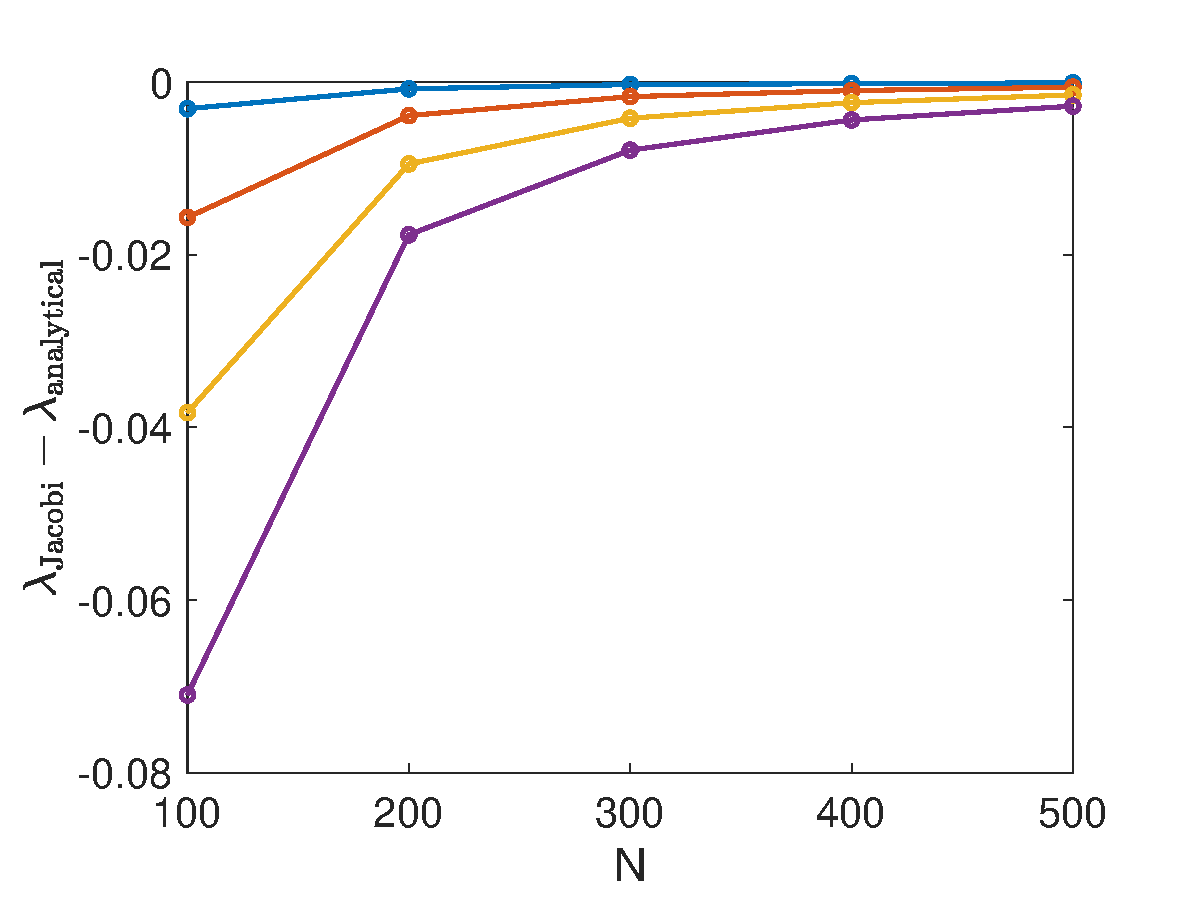
\includegraphics[width=\linewidth]{Jacobi_values.eps}
	\caption{Plot of the difference between the eigenvalues calculated by the Jacobi algorithm and the analytical states for the electron. From top to bottom, $\lambda_\text{analytical} = \{3,7,11,15\}$.}
	\label{fig:jacobi}
\end{figure}

\begin{table}[h]
	\centering
	\caption{For a range of $N$: number of iterations used by Jacobi's algorithm, it's runtime $t_\text{Jacobi}$, and that of Armadillo's ``\texttt{eig\_gen()}'' method $t_\text{arma}$. A fit of the number of iterations to $(a N^2)$ yields $a=1.6$.}
	\label{tab:jacobi}
	\begin{tabular}{|C|C|C|C|}\hline
	N & \text{iterations} & t_\text{Jacobi} [\si{s}] & t_\text{arma} [\si{s}] \\\hline
	100 & 15\,290 & 0.81 & 0.0069\\
	200 & 63\,410 & 12.5 & 0.10\\
	300 & 144\,732 & 66 & 0.25\\
	400 & 259\,167 & 210 & 0.64\\
	500 & 407\,112 & 515 & 0.92\\\hline
	\end{tabular}
\end{table}

Results for Lanczos' algorithm are shown in figure \ref{fig:lanczos}, and a comparison of the runtimes with those of Armadillo's ``\texttt{eig\_gen}'' method are listed in table \ref{tab:lanczos}.

\begin{figure}[h]
	\centering
	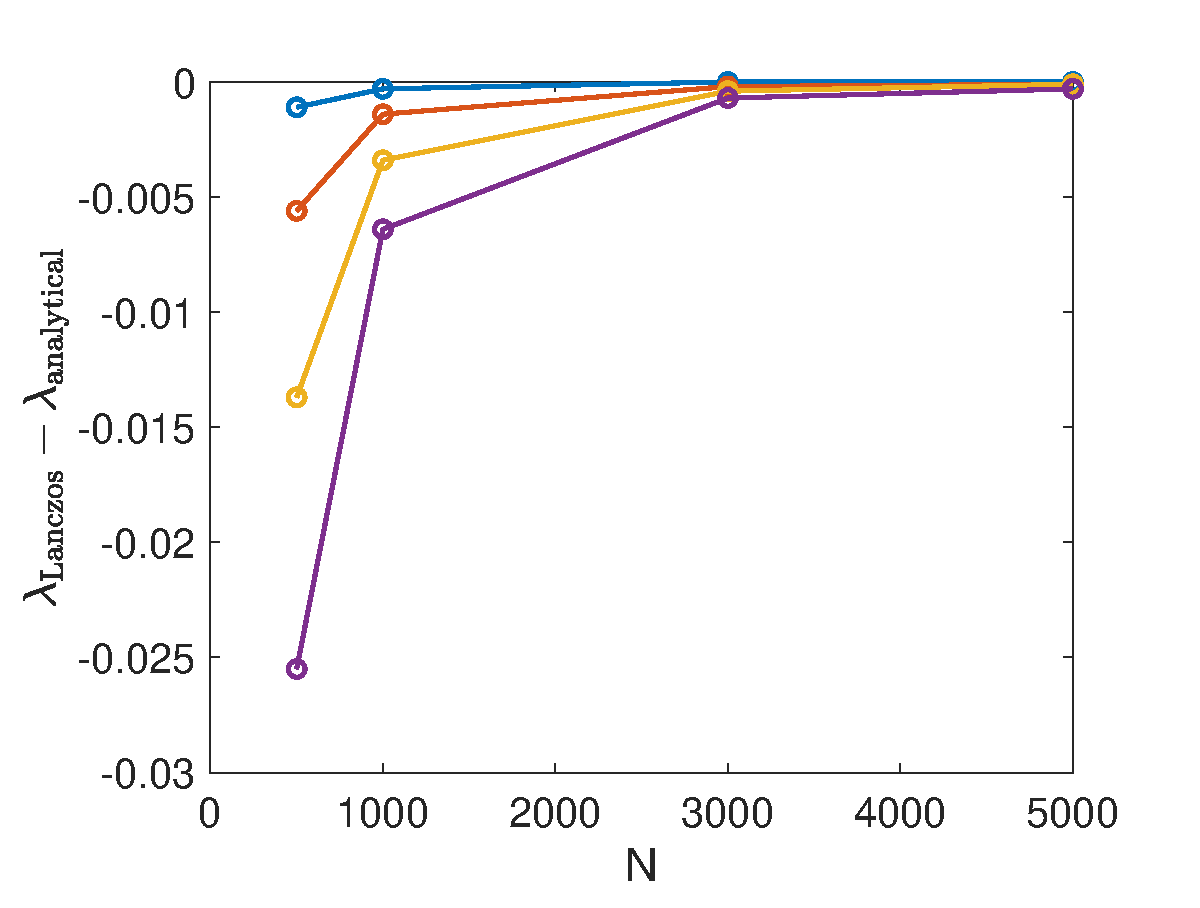
\includegraphics[width=\linewidth]{Lanczos_values.eps}
	\caption{Plot of the difference between the eigenvalues calculated by the Lanczos algorithm with $M=N/5$ iterations and the analytical states for the electron. From top to bottom, $\lambda_\text{analytical} = \{3,7,11,15\}$.}
	\label{fig:lanczos}
\end{figure}



\begin{table}[h]
	\centering
	\caption{For various $N$: runtime of the Lanczos algorithm with $M=N/5$ iterations, and of Armadillo's ``\texttt{eig\_gen()}'' method.}
	\label{tab:lanczos}
	\begin{tabular}{|C|C|C|}\hline
	N & t_\text{Lanczos} [\si{s}] & t_\text{arma} [\si{s}] \\\hline
	500 & 0.029823 & 0.819871\\
	1000 & 0.208129 & 3.34472 \\
	3000 & 5.73699 & 62.5238 \\
	5000 & 48.2992 & 290.692 \\\hline
	\end{tabular}
\end{table}


%
%
%
\section*{Discussion}
In all cases Jacobi's algorithm gives the same result as Armadillo's ``\texttt{eig\_gen()}'' method up to at least four decimal places. This is expected since it diagonalizes the matrix $\vb{A}$ to a tolerance set by us.
The number of iterations for Jacobi's algorithm is of the order of $1.6N^2$. This is slightly less than the expected $3N^2$ to $5N^2$, but still very inefficient compared to \texttt{eig\_gen()}. Our $499\times499$-matrix required 407\,122 iterations and 515\un{s} to diagonalize, whereas Armadillo dit it in $0.9\un{s}$. The higher than expected efficiency might come from the fact that the matrix $\vb{A}$ starts out tridiagonal.  
 
%Jacobi's method is known for being very inefficient, because each transformation might increase matrix elements previously set to zero \cite{lecture}. This inefficiency is confirmed in our experiments. 

With $M=N/5$ iterations, the Lanczos algorithm also gives similar results to Armadillo. However, it can be applied to much larger matrices, allowing for much more accurate estimations of the eigenvalues. It is also much faster, especially for high $N$. This is expected as each iteration only involves one matrix operation, and it only calculates the eigenvalues of a much smaller matrix. The behaviour of Lanczos' algorithm should be compared to quantitative predictions in future work.     

%
%
%
\section*{Conclusion}
We implemented Jacobi's and Lanczos' algorithms and applied them to the eigenvalue problem of a single electron in a harmonic oscillator potential. In both cases we compared the results for the four lowest eigenvalues to the analytical energy levels, and the runtime of the algorithms to that of Armadillo's ``\texttt{eig\_gen()}'' method. While all three methods gave results of similar accuracy for the same $N$, the difference in efficiency meant we could obtain much more accurate values with Lanczos' algorithm by using higher values of $N$.
  
The qualitative behaviour of both algorithms is consistent with theory, though we measured the Jacobi algorithm to be slightly more efficient that expected, likely due to the simplicity of the problem we chose to study. A qualitative comparison with theory for  Lanczos' algorithm is left to future work.



\onecolumn
\begin{thebibliography}{9}

\bibitem{matcomp}
Golub, Gene H., Van Loan, Charles F. (2013) \textit{Matrix Computations}, Fourth edition. Baltimore: The John Hopkins University Press.   

\bibitem{labtext}
Hjort-Jensen, Morten, (2020) \textit{Project 2}, $<$\url{http://compphysics.github.io/ComputationalPhysics/doc/Projects/2020/Project2/html/Project2.html}$>$. 

\bibitem{lecture}
Hjort-Jensen, Morten, (2020) \textit{Computational Physics Lectures: Eigenvalue Problems}, $<$\url{http://compphysics.github.io/ComputationalPhysics/doc/pub/eigvalues/html/eigvalues.html}$>$. 


\end{thebibliography}



% Husk å avslutte alle environments
% SLUTT
\end{document}